\documentclass{beamer}
\mode<presentation>
\usetheme{Ilmenau}
\usepackage{graphics}
\usepackage{mathtools}
\title[Advanced Numerical Methods for Neutron Star Interfaces] % (optional, only for long titles)
{Advanced Numerical Methods for \\
Neutron Star Interfaces}
\subtitle{}
\author[John Muddle - @john$\_$muddle] % (optional, for multiple authors)
{John Muddle}
\institute[University of Southampton] % (optional)
{
  School of Mathematics\\
  University of Southampton\\[1\baselineskip]
  Supervisor - Ian Hawke

}
\date[Britgrav 2016] % (optional)
{BritGrav, 2016}
\AtBeginSection[]
{
  \begin{frame}<beamer>
    \frametitle{Outline}
    \tableofcontents[currentsection]
  \end{frame}
}
\begin{document}


\begin{frame}
  \titlepage
\end{frame}
\begin{frame}
\frametitle{Acknowledgements}
I would like to thank the following:
\begin{itemize}
\item{Ian Hawke}
\item{Southampton General Relativity Group}
\item{STFC}
\item{IOP Gravity Group}
\item{Classical and Quantum Gravity}
\end{itemize}
\end{frame}
 \begin{frame}
   \frametitle{Outline}
   \tableofcontents
 \end{frame}
\section{Motivation: Neutron Stars}

\begin{frame}
\frametitle{Motivation: Binary Mergers}
\begin{columns}
\column{0.55\textwidth}
\begin{itemize}
\item{Neutron star binary mergers are strong candidates for the emission of detectable gravitational waves.}
\item{Accurate gravitational wave templates are required to directly detect gravitational waves.}
\item{Full non-linear numerical simulations are required for the plunge and merger phases.}
\item{Therefore, accurate numerical simulations are needed.}
\end{itemize}
\column{0.45\textwidth}
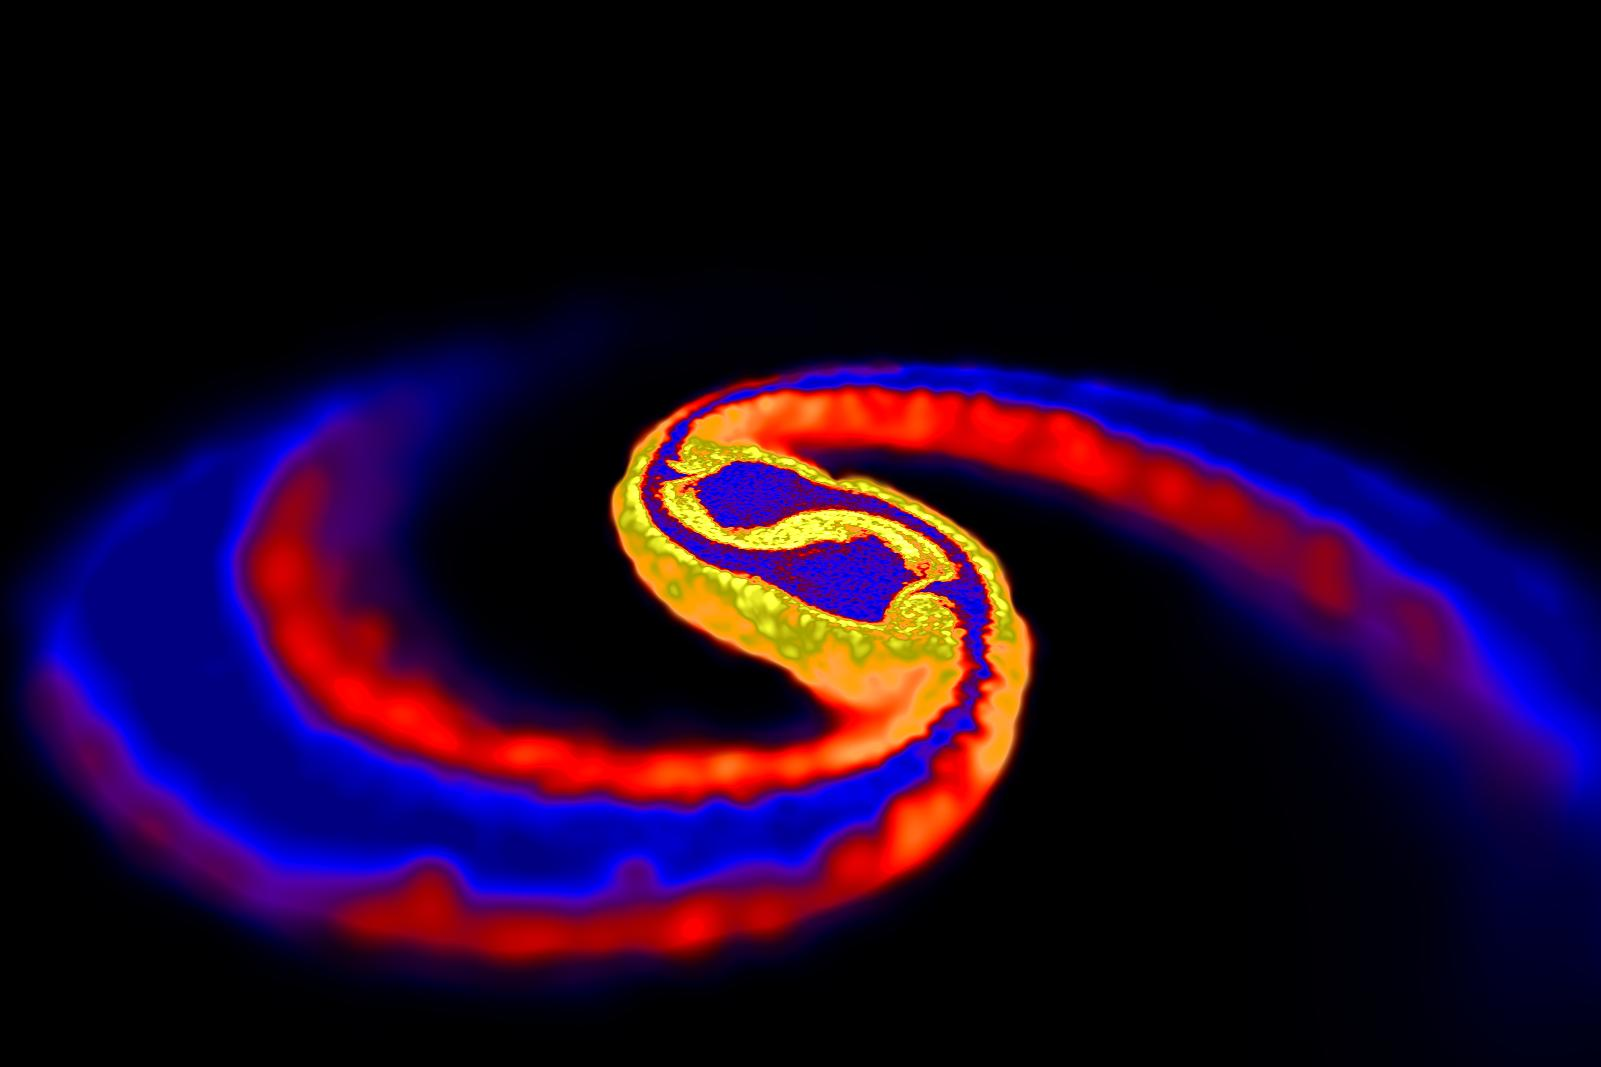
\includegraphics[width=\textwidth]{../images/price_rosswog_press_1}\\
\tiny Credit: Daniel Price (U/Exeter) and Stephan Rosswog (Int. U/Bremen)
\end{columns}
\end{frame}

%\begin{frame}
%\frametitle{Neutron Star Structure: Internal}
%\begin{columns}[T]
%\column{6.5cm}
%\centering
%\includegraphics[width=6.5cm]{images/neutron_star_structure}
%\column{4cm}
%Consider a NS close to merger.
%\begin{itemize}
%\item{The star is old and cold.}
%\item{The core can be approximated as a perfect fluid.}
%\item{The crust can be approximated as elastic matter.}
%\end{itemize}
%\end{columns}
%\end{frame}


%\begin{frame}
%\frametitle{Neutron Star Structure: Electromagnetic}
%\begin{columns}[T]
%\column{6.5cm}
%\centering
%\includegraphics[width=6.5cm]{images/neutron_star_magnetic}
%\column{4.0cm}
%Goldreich-Julian magnetosphere
%\begin{itemize}
%\item{Predominately dipolar.}
%\item{Polodial and toroidal components.}
%\item{Radial beyond light cylinder.}
%\end{itemize}
%\end{columns}
%\end{frame}


\section{How do we model a neutron star?}
\begin{frame}
\frametitle{What features do we need to consider?}
\begin{columns}
\column{0.5\textwidth}
\begin{itemize}
\item{Exterior - Vacuum/Plasma}
\item{Atmosphere - Fluid}
\item{Crust - Elastic Matter}
\item{Core - Fluid}
\end{itemize}
\column{0.6\textwidth}
\includegraphics[width=\textwidth]{../images/neutron_star_structure}
\end{columns}
\end{frame}
\begin{frame}
\frametitle{How do we model a neutron star numerically?}
We want to solve the most realistic physical model possible using maximum resolution. Problem?
\begin{itemize}
\item{Important length-scales vary over 12 orders of magnitude if including viscous boundary layers.}
\item{Using adaptive mesh refinement cannot cover this range.}
\end{itemize}
Solution: \\
Relativistic multimodel approach developed by Millmore \& Hawke. \\
Approximate interfaces to be infinitely thin.
\end{frame}

\begin{frame}
\frametitle{The multimodel approach}
Simplify the most complex model by:
\begin{itemize}
\item{Taking appropriate limits in different regions of the domain.}
\begin{itemize}
\item{Force-free / Electro-vacuum / Multi-fluid MHD}
\item{Ideal MHD / Resistive MHD}
\item{Elasticity}
\end{itemize}
\item{Combining the different approximations with sharp interfaces.}
\item{Using evolution equations based on conservation laws.}
\begin{itemize}
\item{This allows us to accurately capture the locations of shock waves}
\end{itemize}
\item{Moving the complicated physics to the interfaces.}
\begin{itemize}
\item{Boundary conditions to impose physics}
\end{itemize}
\end{itemize}
This approach also allows a proper treatment of the surface. \\
Therefore, we no longer need a numerical atmosphere. 
\end{frame}

%\begin{frame}
%\frametitle{Conservation Laws}
%\centering
%$\frac{\partial \bf{q}(x,t)}{\partial x}  + \frac{\partial F(q(x,t))}{\partial x} = 0.$ 
%$q^{n+1}_i = q^n_i + \frac{\Delta t}{\Delta x} \left(F^n_{i-1/2} + F^n_{i+1/2}\right)$ 
%
%\end{frame}
\begin{frame}
\frametitle{Conservation Laws}
The evolution equations are a system of non-linear partial differential equations in conservation law form.
\begin{equation}
\frac{\partial \mathbf{q}(x,t)}{\partial x}  + \frac{\partial \mathbf{F}(\mathbf{q}(x,t))}{\partial x} = 0,
\end{equation}
where $\mathbf{q}$ are the conserved variables and $\mathbf{F}$ are the fluxes.\\
The numerical update is then given by.
\begin{equation}
q^{n+1}_i = q^n_i + \frac{\Delta t}{\Delta x} \left(F^n_{i-1/2} - F^n_{i+1/2}\right),
\end{equation}
where $n$ is the time index and $i$ is the spatial index.
\end{frame}

\begin{frame}
\frametitle{Numerical Grid}
\begin{columns}
\column{0.45\textwidth}
\begin{itemize}
\item{We define a grid on which to evolve our models}
\item{The red line indicates the true interface}
\item{The white line indicates the numerical interface}
\end{itemize}
\column{0.55\textwidth}
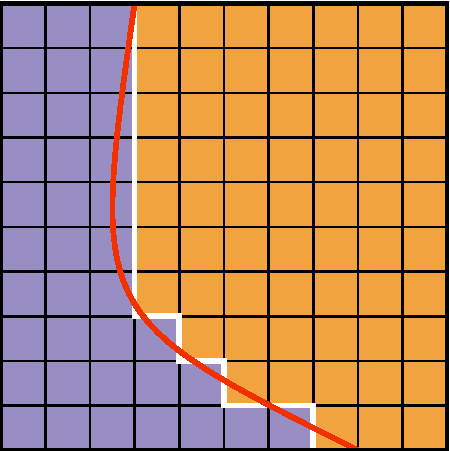
\includegraphics[width=\textwidth]{../images/multimodel_captured.pdf}
\end{columns}
\end{frame}

\begin{frame}
\frametitle{Moving Interface}
\begin{columns}
\column{0.45\textwidth}
\begin{itemize}
\item{The interface is advected with the models}
\item{The numerical interface tracks the physical interface}
\item{Points can change model}
\end{itemize}
\column{0.55\textwidth}
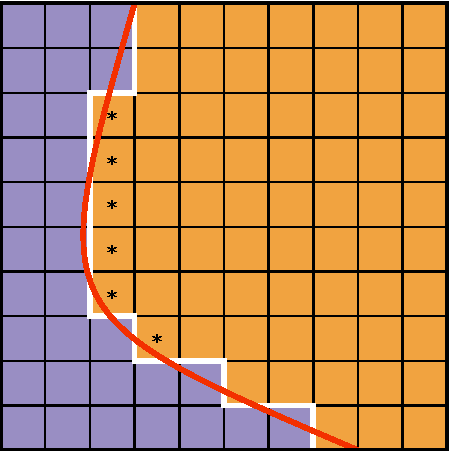
\includegraphics[width=\textwidth]{../images/multimodel_captured_2.pdf}
\end{columns}
\end{frame}

\begin{frame}
\frametitle{Ghost Zones}
\begin{columns}
\column{0.45\textwidth}
\begin{itemize}
\item{Each model has a region of ghost zones}
\item{As the update of each point is non-local, it is important to fill these cells correctly}
\item{How do we impose the correct boundary conditions? By filling the ghost cells}
\end{itemize}
\column{0.55\textwidth}
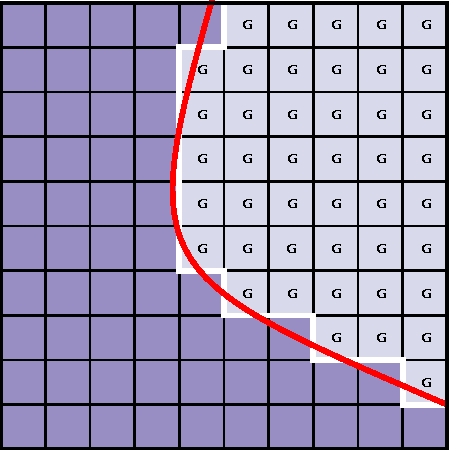
\includegraphics[width=\textwidth]{../images/multimodel_ghostcells.pdf}
\end{columns}
\end{frame}

\begin{frame}
\frametitle{Riemann Problem and Solution}
\begin{columns}
\column{0.5\textwidth}
\begin{itemize}
\item{Each normal cell is updated by following the Godunov approch}
\item{Each cell boundary is a Riemann problem}
\item{A Riemann problem occurs when there is discontinuity}
\item{We update each cell by calculating the flux through the boundaries}
\end{itemize}
\column{0.6\textwidth}
\centering
Hydro Riemann Fan
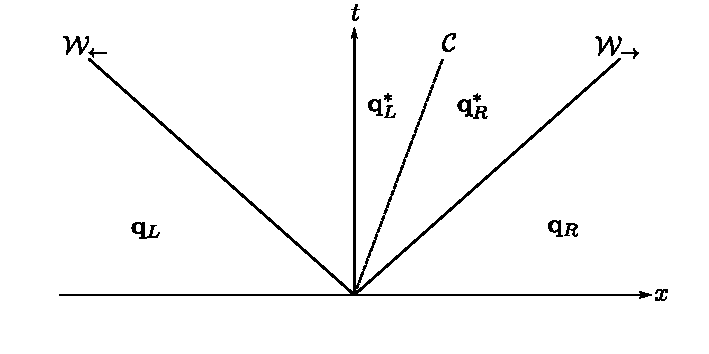
\includegraphics[width=\textwidth]{../images/euler_wave.pdf}
\end{columns}
\end{frame}

\begin{frame}
\frametitle{Riemann Problem and Solution}
\begin{columns}
\column{0.5\textwidth}
\begin{itemize}
\item{Each normal cell is updated by following the Godunov approach}
\item{Each cell boundary is a Riemann problem}
\item{A Riemann problem occurs when there is discontinuity}
\item{We update each cell by calculating the flux through the boundaries}
\end{itemize}
\column{0.6\textwidth}
\centering
SRMHD Riemann Fan
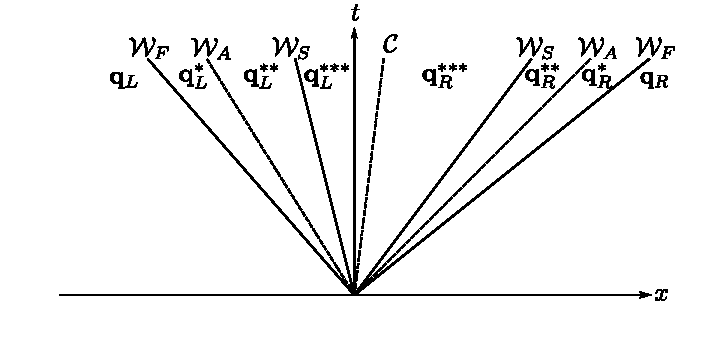
\includegraphics[width=\textwidth]{../images/srmhd_wave.pdf}
\end{columns}
\end{frame}

\section{Interfaces and Boundary Conditions}

%\begin{frame}
%\frametitle{Splitting the domain}
%\begin{columns}
%\column{7.5cm}
%\centering
%\includegraphics[width=7.5cm]{images/multimodel_domain}
%\column{3.5cm}
%Each model has it's own domain $\Omega_m$ and a boundary $\partial\Omega_m$.
%\end{columns}
%\end{frame}

%\begin{frame}
%\frametitle{Tracking the Interface}
%We use a scalar level-set function $\phi$ to track the interface between two different models:
%\begin{columns}
%\column{5cm}
%\begin{itemize}
%\item{The level set is evolved by solving a Hamilton-Jacobi equation.}
%\item{The interface location is advected along with the physical velocity.}
%\item{Each model has its own level-set.}
%\end{itemize}
%\column{5cm}
%\includegraphics[width=5cm]{images/levelset}
%\end{columns}
%\end{frame}


\begin{frame}{Boundary Conditions: Ghost Fluid Method}
\begin{columns}
\column{6.5cm}
\centering
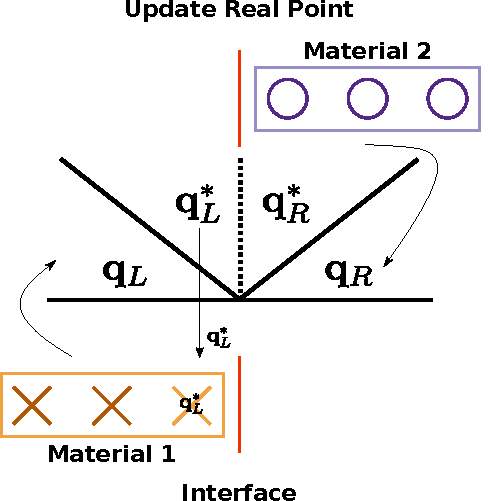
\includegraphics[width=6.5cm]{../images/multimodel_roe_real}
\column{4.5cm}
Follow the ghost fluid approach.
\begin{itemize}
\item{Define left and right states.}
\item{Calculate the star states using an appropriate method.}
\item{Fill the points neighbouring the interface.}
\item{Extrapolate into the ghost zones.}
\end{itemize}
\end{columns}
\end{frame}
\begin{frame}{Boundary Conditions: Ghost Fluid Method}
\begin{columns}
\column{6.5cm}
\centering
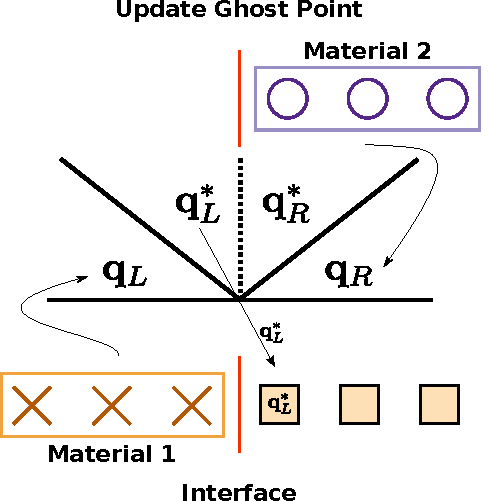
\includegraphics[width=6.5cm]{../images/multimodel_roe_ghost}
\column{4.5cm}
Follow the ghost fluid approach.
\begin{itemize}
\item{Define left and right states.}
\item{Calculate the star states using an appropriate method.}
\item{Fill the points neighbouring the interface.}
\item{Extrapolate into the ghost zones.}
\end{itemize}
\end{columns}
\end{frame}
\begin{frame}{Boundary Conditions: Ghost Fluid Method}
\begin{columns}
\column{6.5cm}
\centering
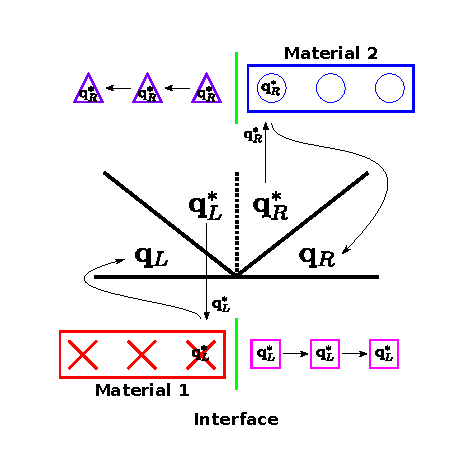
\includegraphics[width=6.5cm]{../images/multimodel_roe}
\column{4.5cm}
Follow the ghost fluid approach.
\begin{itemize}
\item{Define left and right states.}
\item{Calculate the star states using an appropriate method.}
\item{Fill the points neighbouring the interface.}
\item{Extrapolate into the ghost zones.}
\end{itemize}
\end{columns}
\end{frame}

\begin{frame}
\frametitle{How do we calculate the star states?}
To calculate the star states we follow the Roe approximation method and linearise about an appropriate state $\mathbf{w}_X(\mathbf{q}_X)$ for the left and right states. Where $X = L/R$.
\begin{equation}
\partial_t\mathbf{w}_X + \hat{A}_X\partial_{\mathnormal{x}}\mathbf{w}_X = 0.
\end{equation}
The star states are then given by the following equations.
\begin{align}
\mathbf{w}^*_L &= \mathbf{w}_L+\sum^{N_L}_{i=1}c^L_{i}\mathbf{r}^{(i)}_L,\\
\mathbf{w}^*_R &= \mathbf{w}_R-\sum^{N_R}_{j=1}c^R_{j}\mathbf{r}^{(j)}_R.
\end{align}
Where $\mathbf{r}_X$ are the right eigenvectors of the matrix $\hat{A}_X$.
\end{frame}

\begin{frame}
\frametitle{How do we impose the interface boundary conditions?}
To calculate the coefficients $c^X$ we need  $N = N_L + N_R$ compatibility conditions at the interface. Where $N_X$ is the number of waves between the initial and star state.\\
It is through these compatibility conditions that we impose the correct physical boundary conditions at the interface.\\
We assume that these compatibility conditions take the form:

\begin{equation}
\Delta w_j = w^{*R}_j-w^{*L}_j = 0, \quad j = 1,\dots, N.
\end{equation}
This gives a linear system which we can easily solve,
\begin{equation}
\mathbf{w}_R - \mathbf{w}_L = \sum^{N_R}_{j=1}c^R_{j}\mathbf{r}^{(j)}_R +  \sum^{N_L}_{i=1}c^L_{i}\mathbf{r}^{(i)}_L.
\end{equation}
\end{frame}

\section{Results}

\begin{frame}
\frametitle{Vorticity Propagation - Low Magnetic Field $\beta = 1000$}
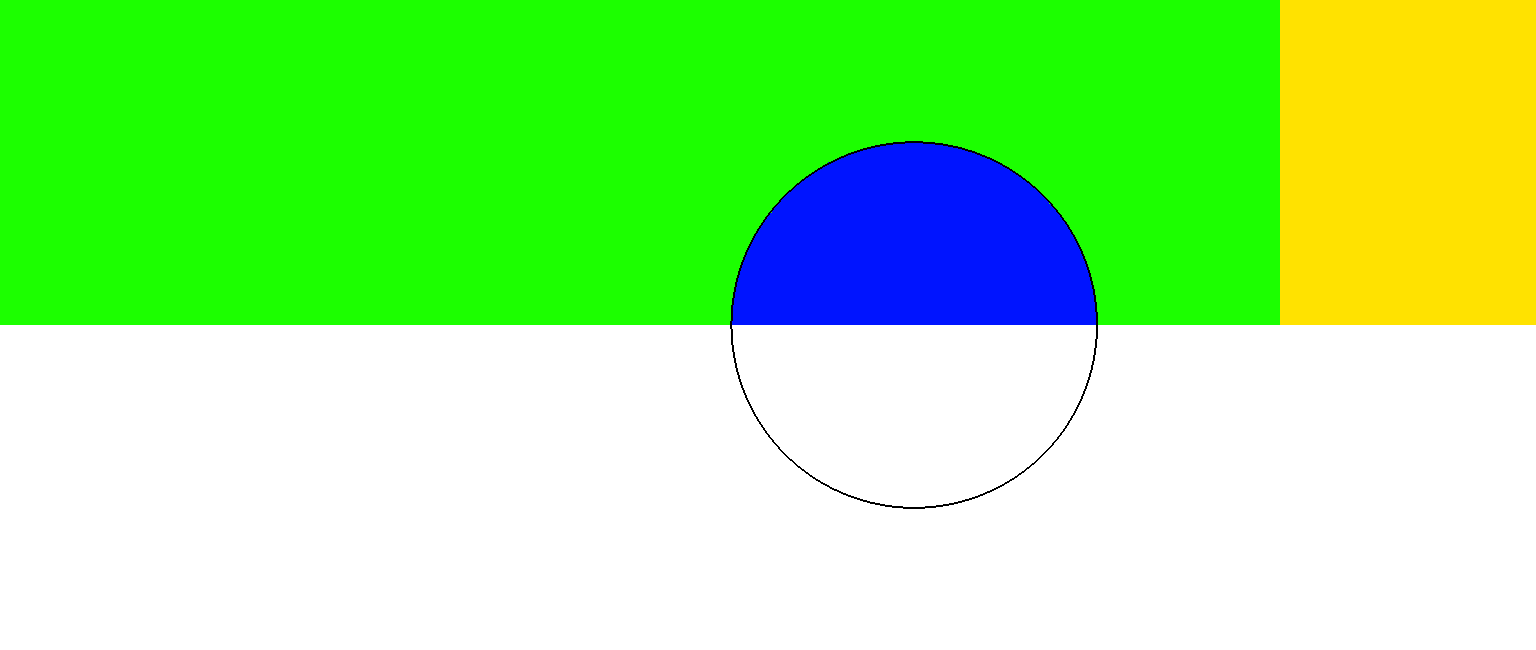
\includegraphics[width=\textwidth]{../images/SRMHDBubbleBeta1000_t0_crop.png}
\end{frame}

\begin{frame}
\frametitle{Vorticity Propagation - Low Magnetic Field $\beta = 1000$}

\includegraphics[width=\textwidth]{../images/SRMHDBubbleBeta1000_t31_crop.png}
\end{frame}

\begin{frame}
\frametitle{Vorticity Propagation - Low Magnetic Field $\beta = 1000$}
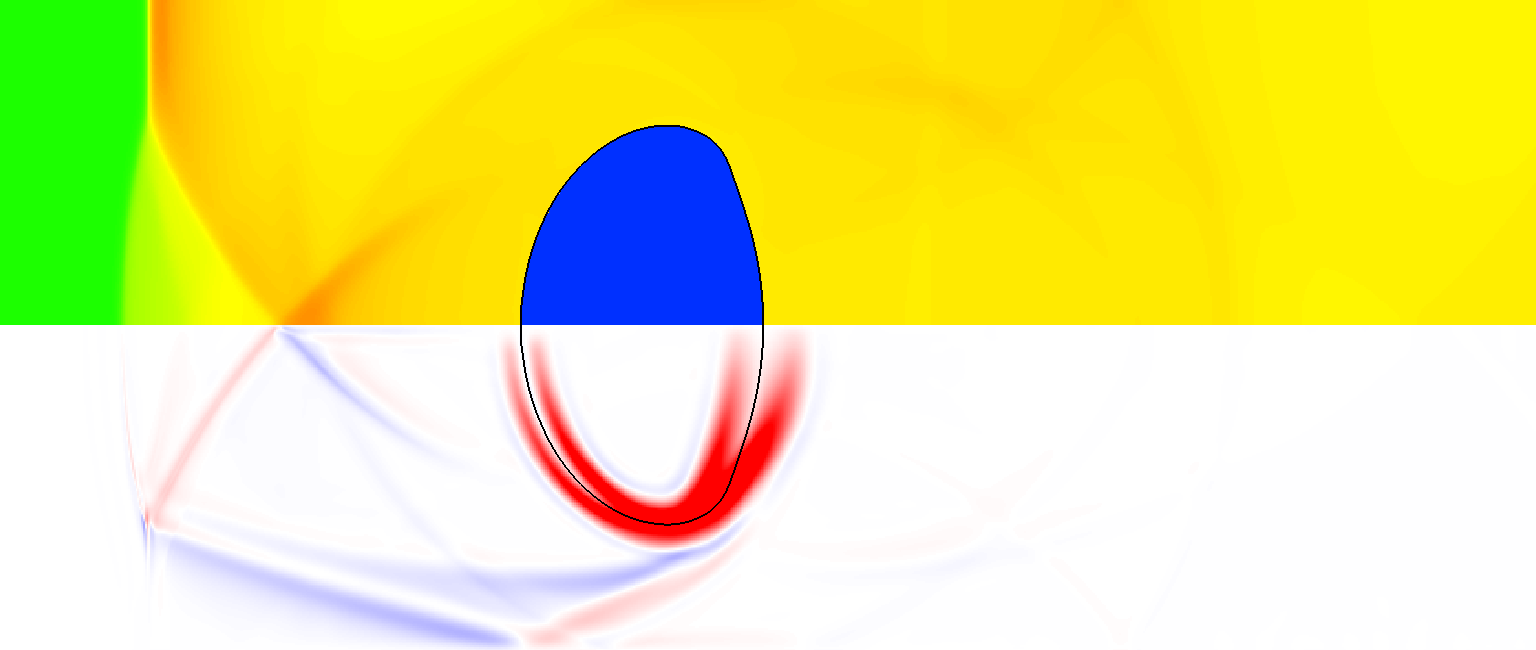
\includegraphics[width=\textwidth]{../images/SRMHDBubbleBeta1000_t59_crop.png}
\end{frame}

\begin{frame}
\frametitle{Vorticity Propagation - Low Magnetic Field $\beta = 1000$}
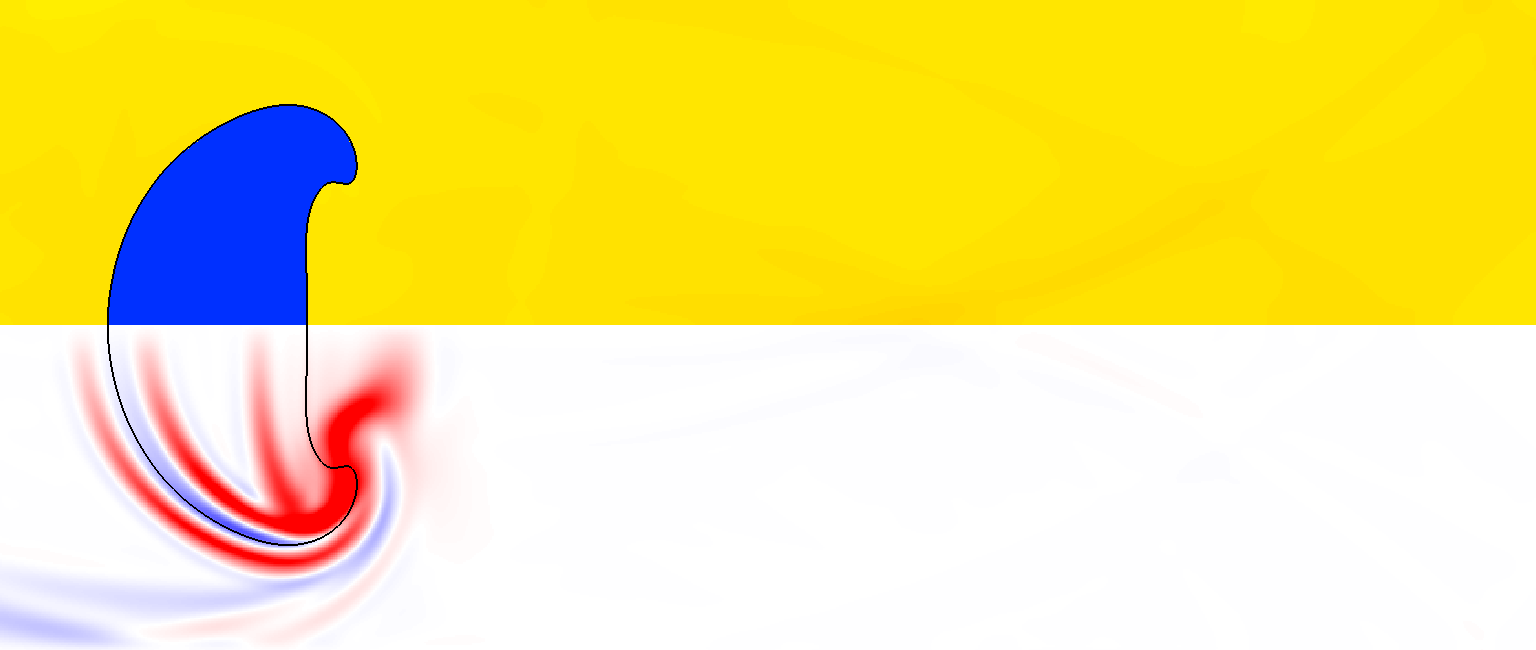
\includegraphics[width=\textwidth]{../images/SRMHDBubbleBeta1000_t125_crop.png}
\end{frame}

\begin{frame}
\frametitle{Vorticity Propagation - Low Magnetic Field $\beta = 0.01$}
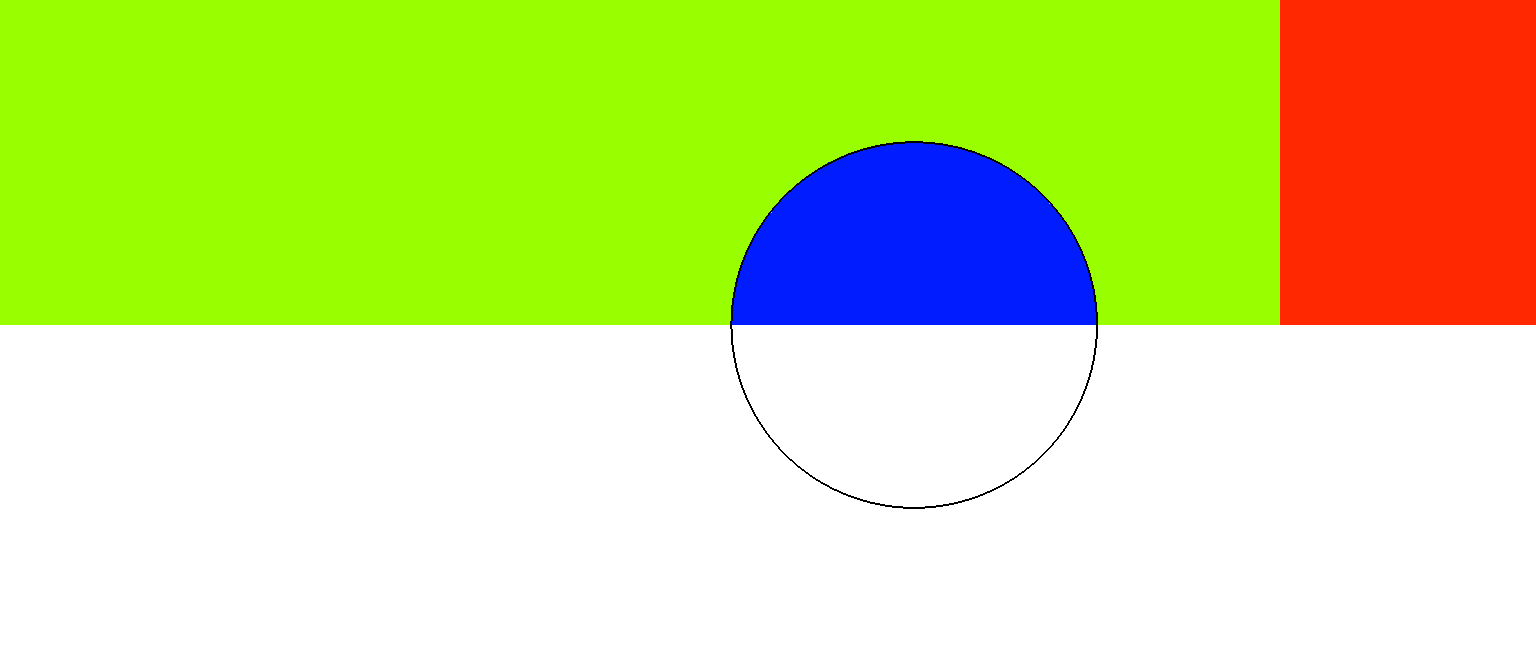
\includegraphics[width=\textwidth]{../images/SRMHDBubbleBeta001_t0_crop.png}
\end{frame}

\begin{frame}
\frametitle{Vorticity Propagation - Low Magnetic Field $\beta = 0.01$}
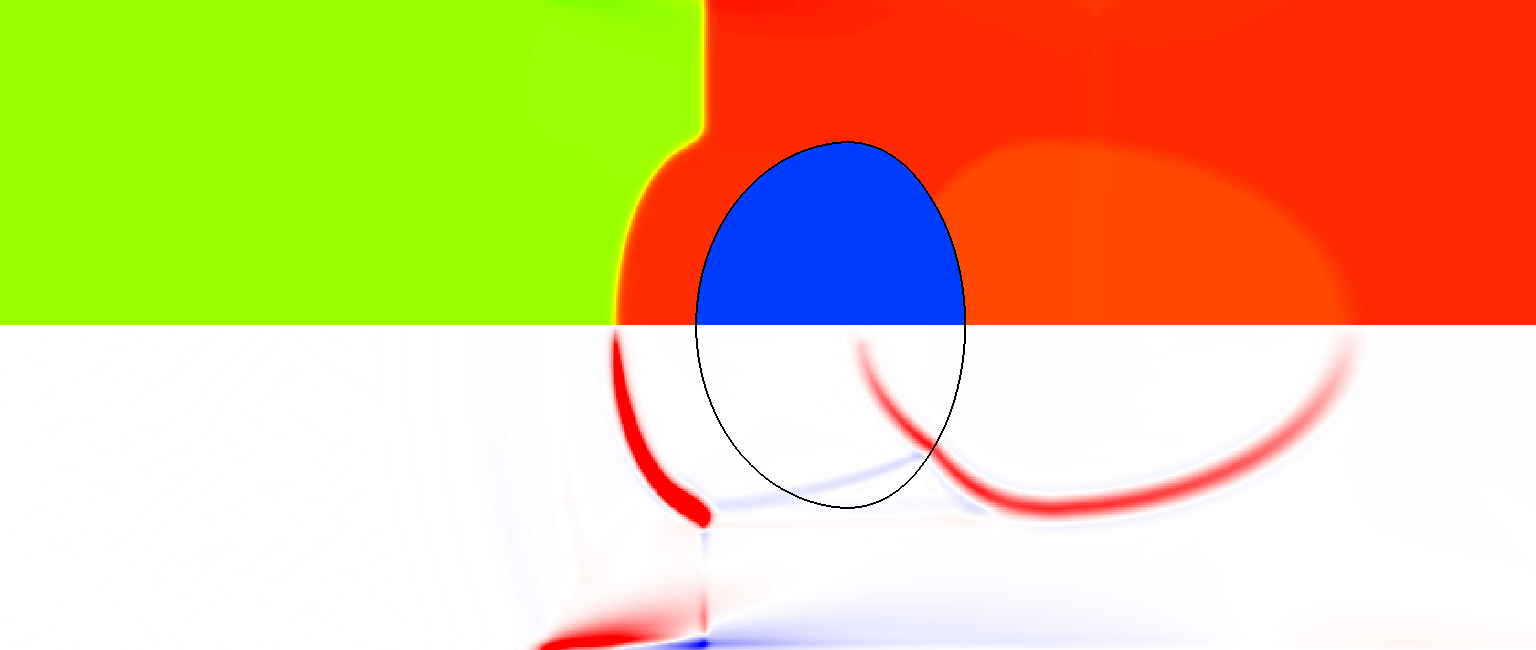
\includegraphics[width=\textwidth]{../images/SRMHDBubbleBeta001_t31_crop.png}
\end{frame}

\begin{frame}
\frametitle{Vorticity Propagation - Low Magnetic Field $\beta = 0.01$}
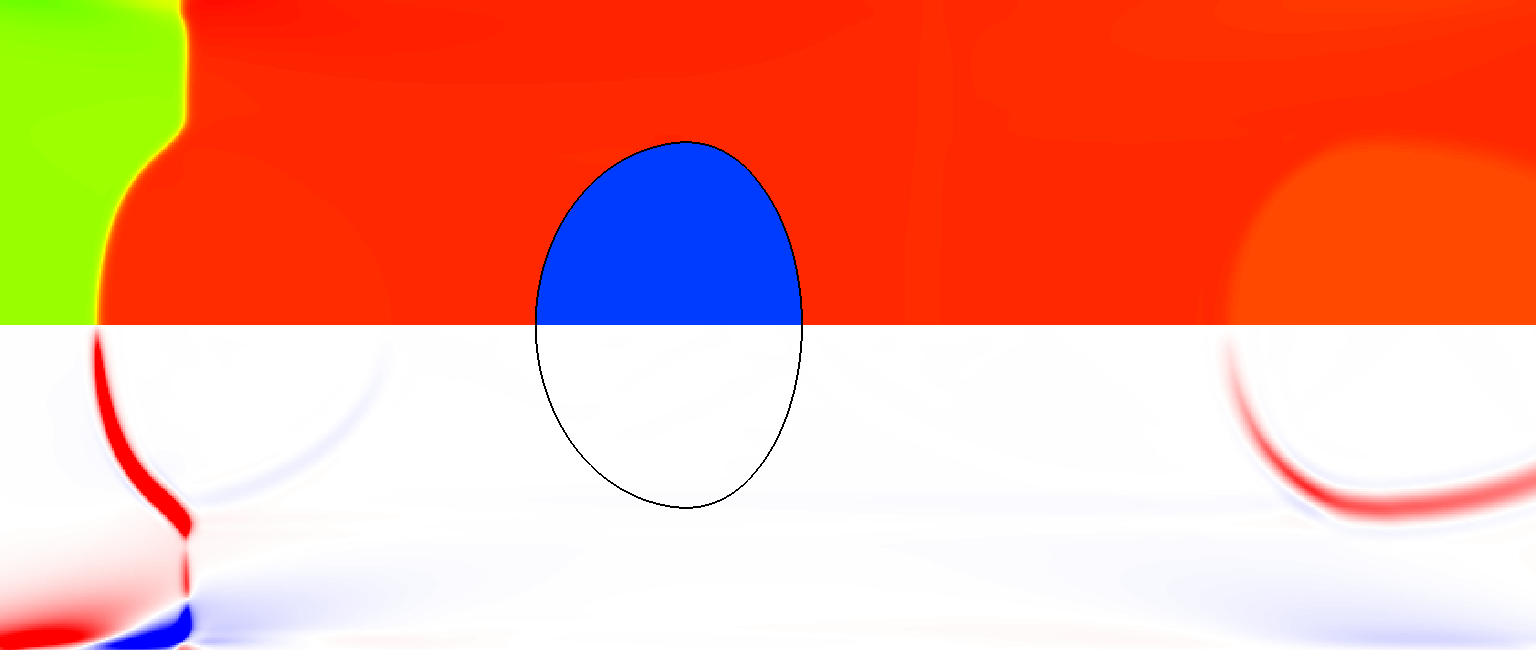
\includegraphics[width=\textwidth]{../images/SRMHDBubbleBeta001_t59_crop.png}
\end{frame}

\begin{frame}
\frametitle{Vorticity Propagation - Low Magnetic Field $\beta = 0.01$}
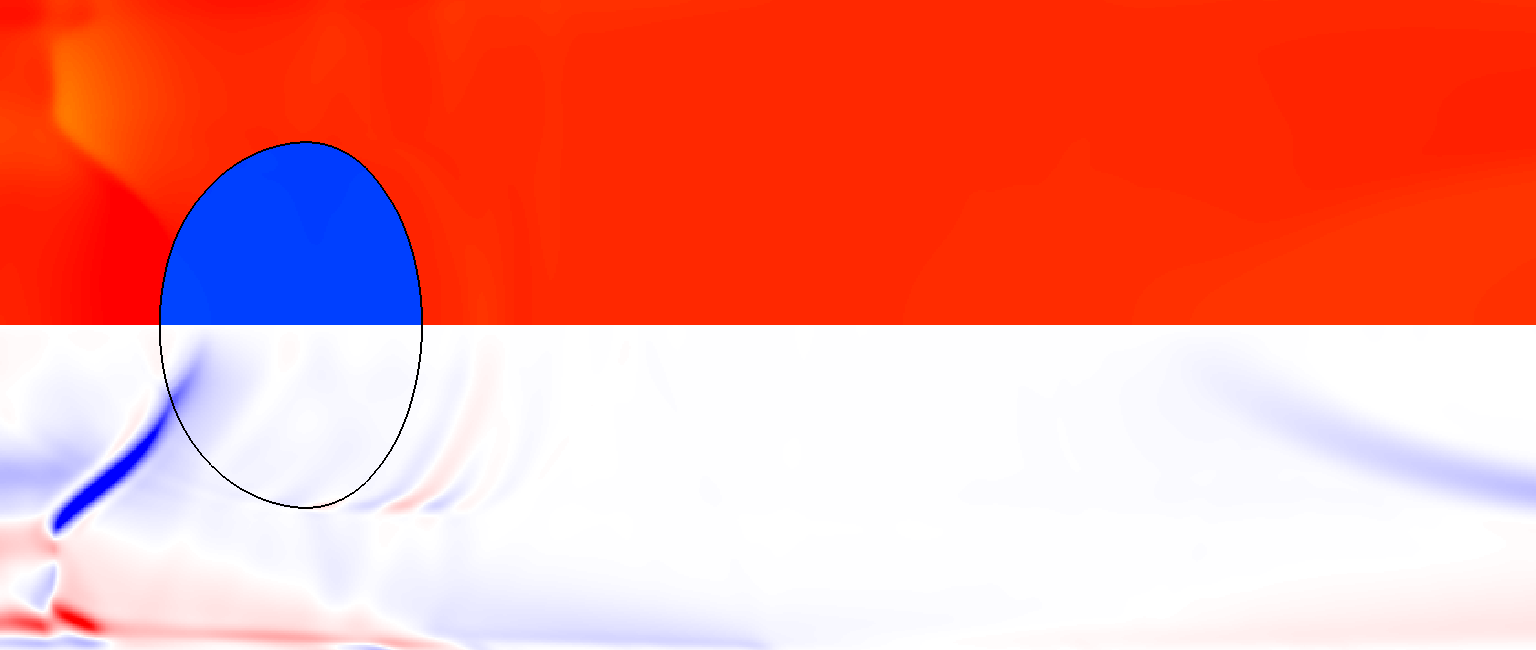
\includegraphics[width=\textwidth]{../images/SRMHDBubbleBeta001_t125_crop.png}
\end{frame}

\begin{frame}
\frametitle{Toy Star: Vacuum - Hydro}
\centering
\includegraphics[width=0.65\textwidth]{../images/toy_density}
\end{frame}
\begin{frame}
\frametitle{Toy Star: Vacuum - Hydro}
\centering
\includegraphics[width=0.7\textwidth]{../images/toy_velocity}
\end{frame}
\begin{frame}
\frametitle{Toy Star: Vacuum - Hydro}
\centering
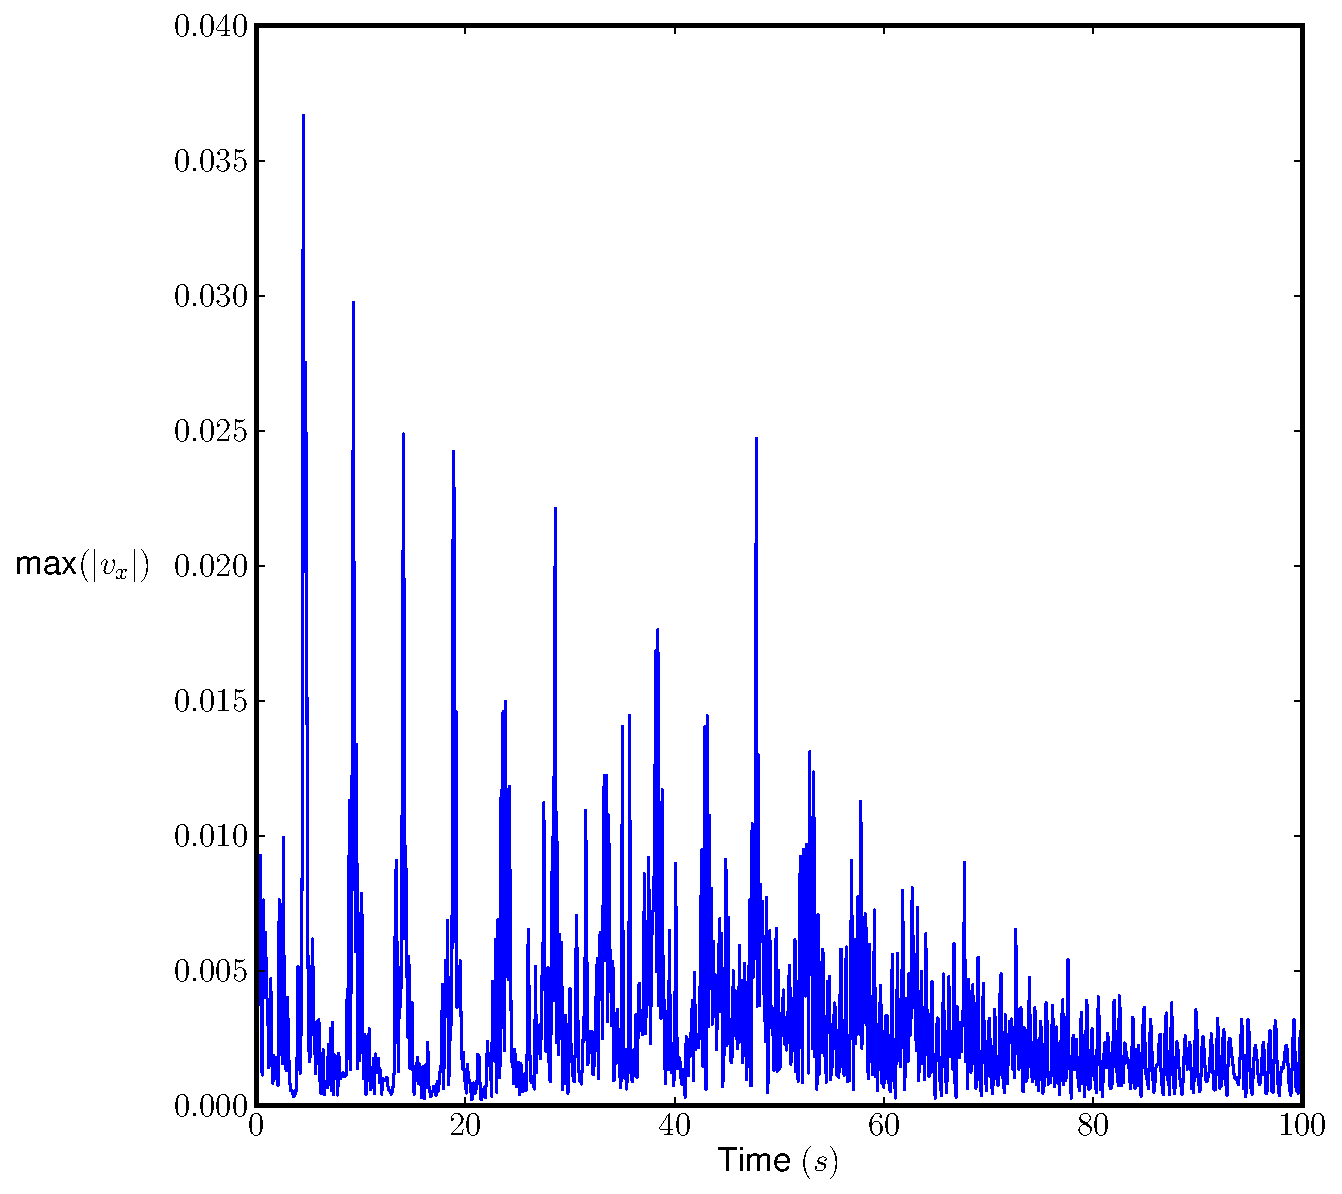
\includegraphics[width=0.7\textwidth]{../images/toy_max_vx}
\end{frame}

\section{Conclusion}
\begin{frame}
\frametitle{Conclusion}
Thank you
\end{frame}
\end{document}

%\begin{frame}
%\frametitle{How do we impose the interface boundary conditions}
%In the case of a Hydro-Hydro interface problem we $N=2$ compatibility conditions.\\
%What physical conditions do we impose?
%\begin{itemize}
%\item{Continuity of traction}
%\end{itemize}
%\begin{align}
%\Delta p &= 0, \\
%\Delta v^n &= 0.
%\end{align}
%The pressure and normal velocity are continuous across the interface.
%\end{frame}

%\section{Surface Treatment}
%\begin{frame}
%\frametitle{What happens at the surface?}
%How to do we include the surface of the neutron star?
%\begin{itemize}
%\item{Current simulations set an atmosphere floor when cells evolve to an unphysical state.}
%\item{Typically, this atmosphere is 8 to 10 orders of magnitude lower than the central density [Reisswig 2013].}
%\item{We want to treat the surface as an interface and apply the Roe approximation method.}
%\item{This should allow us to accurately track the surface and have a true vacuum exterior.}
%\end{itemize}
%\end{frame}
%
%\begin{frame}
%\frametitle{Surface Treatment}
%How do we apply the Roe approximation method here?\\
%Consider the following situation: Hydro-Vacuum.\\
%\centering
%%\includegraphics[width=8cm]{images/toy_wave}\\
%\raggedright
%\end{frame}
%
%\begin{frame}
%\frametitle{What are the physical boundary conditions?}
%At the surface we expect the pressure and density to go to zero. \\
%We have the following primitive states:
%\begin{align}
%\mathbf{w}_L &= \{\rho, v^n, p\},\\
%\mathbf{w}_R&=\{0\}.
%\end{align}
%However, if we use both the pressure and the density then the problem is ill-posed. This is because we are only allowed one compatibility condition as there is only a single wave. \\
%Therefore, we need a new set of variables that are well-posed.
%\end{frame}
%
%\begin{frame}
%\frametitle{What are the appropriate variables?}
%For a polytropic equation of state the following relation is true, 
%\begin{equation}
%p = K \rho^{\gamma}.
%\end{equation}
%Therefore, we can fix the effective entropy $K$ at the surface. \\
%This gives us the following states,
%\begin{equation}
%\mathbf{w}_L = \{p,v^n,K\}, \quad \mathbf{w}_R = \{0\},
%\end{equation}
%and a single compatibility condition
%\begin{equation}
%\Delta p = 0.
%\end{equation}
%The resulting coefficient $c_L$ and eigenvector $\mathbf{r}_L$ are given by
%\begin{equation}
%c_L = \dfrac{p^{\frac{\gamma - 1}{2\gamma}}K^{\frac{1}{2\gamma}}}{\sqrt{\gamma}} \quad \mathbf{r}_L = \left\{-p^{\frac{1+\gamma}{2\gamma}}\sqrt{\gamma}K^{\frac{-1}{2\gamma}},1,0\right\}.
%\end{equation}
%\end{frame}
%
%\section{Toy Star}
%\begin{frame}
%\frametitle{Test: Toy Star}
%To validate our surface approach we apply it to a toy star [Price 2004].\\
%We augment the Euler equations with the following source terms,
%\begin{align}
%\partial_t \rho + \partial_x (\rho v) &= 0,\\
%\partial_t (\rho v) + \partial_x(\rho v^2 + p) &= -\rho x, \\
%\partial_t E + \partial_x([E+p]v) &= -\rho v x.
%\end{align}
%The following initial conditions produces a static star in a potential when $\gamma = 2$.
%\begin{align}
%\rho_0 &= (1-x^2),\\
%v_0 &= 0, \\
%p_0   &= \dfrac{\rho_0^\gamma }{4\rho_0(\gamma-1)}.
%\end{align}
%\end{frame}
%
%\begin{frame}
%\frametitle{Results: Toy Star}
%\begin{columns}
%\column{7.5cm}
%\centering
%%\includegraphics[width=7.0cm]{images/toy_density}
%\column{4.5cm}
%Results for a 400 point simulation. 
%\begin{itemize}
%\item{Initial density maximum below 1.0 due to discretisation.}
%\item{Maximum density then oscillates around 1.0.}
%\item{The density floor is set 14 orders of magnitude lower than the central density.}
%\end{itemize}
%\end{columns}
%\end{frame}
%
%\begin{frame}
%\frametitle{Results: Toy Star}
%\begin{columns}
%\column{7.5cm}
%\centering
%%\includegraphics[width=7.0cm]{images/toy_velocity}
%\column{4.5cm}
%\begin{itemize}
%\item{Due to numerical error the initial data is not static and the star expands.}
%\item{Velocity error reduces with increased resolution.}
%\item{The surface of the star oscillates.}
%\end{itemize}
%\end{columns}
%\end{frame}
%\begin{frame}
%\frametitle{Conclusion}
%Where do we stand?
%\begin{itemize}
%\item{Initial results are encouraging - stable and robust.}
%\item{More results required to show convergence and damping of maximum velocity.}
%\item{Extension to SR and the inclusion of magnetic fields needed.}
%\item{Apply to the aligned rotator problem to compare with other published results [Paschalidis 2013, Palenzuela 2013]. }
%\end{itemize}
%\centering
%Any Questions?
%\end{frame}
